% setwd("SpecificationSims/Writeup/")
\documentclass{article}
\usepackage{graphicx, color}
\IfFileExists{upquote.sty}{\usepackage{upquote}}{}
\definecolor{fgcolor}{rgb}{0.267, 0.267, 0.267}
\newcommand{\hlnumber}[1]{\textcolor[rgb]{0,0,0}{#1}}%
\newcommand{\hlfunctioncall}[1]{\textcolor[rgb]{0.501960784313725,0,0.329411764705882}{\textbf{#1}}}%
\newcommand{\hlstring}[1]{\textcolor[rgb]{0.6,0.6,1}{#1}}%
\newcommand{\hlkeyword}[1]{\textcolor[rgb]{0,0,0}{\textbf{#1}}}%
\newcommand{\hlargument}[1]{\textcolor[rgb]{0.690196078431373,0.250980392156863,0.0196078431372549}{#1}}%
\newcommand{\hlcomment}[1]{\textcolor[rgb]{0.180392156862745,0.6,0.341176470588235}{#1}}%
\newcommand{\hlroxygencomment}[1]{\textcolor[rgb]{0.43921568627451,0.47843137254902,0.701960784313725}{#1}}%
\newcommand{\hlformalargs}[1]{\textcolor[rgb]{0.690196078431373,0.250980392156863,0.0196078431372549}{#1}}%
\newcommand{\hleqformalargs}[1]{\textcolor[rgb]{0.690196078431373,0.250980392156863,0.0196078431372549}{#1}}%
\newcommand{\hlassignement}[1]{\textcolor[rgb]{0,0,0}{\textbf{#1}}}%
\newcommand{\hlpackage}[1]{\textcolor[rgb]{0.588235294117647,0.709803921568627,0.145098039215686}{#1}}%
\newcommand{\hlslot}[1]{\textit{#1}}%
\newcommand{\hlsymbol}[1]{\textcolor[rgb]{0,0,0}{#1}}%
\newcommand{\hlprompt}[1]{\textcolor[rgb]{0.266666666666667,0.266666666666667,0.266666666666667}{#1}}%

\usepackage{color}%
 
\newsavebox{\hlnormalsizeboxclosebrace}%
\newsavebox{\hlnormalsizeboxopenbrace}%
\newsavebox{\hlnormalsizeboxbackslash}%
\newsavebox{\hlnormalsizeboxlessthan}%
\newsavebox{\hlnormalsizeboxgreaterthan}%
\newsavebox{\hlnormalsizeboxdollar}%
\newsavebox{\hlnormalsizeboxunderscore}%
\newsavebox{\hlnormalsizeboxand}%
\newsavebox{\hlnormalsizeboxhash}%
\newsavebox{\hlnormalsizeboxat}%
\newsavebox{\hlnormalsizeboxpercent}% 
\newsavebox{\hlnormalsizeboxhat}%
\newsavebox{\hlnormalsizeboxsinglequote}%
\newsavebox{\hlnormalsizeboxbacktick}%

\setbox\hlnormalsizeboxopenbrace=\hbox{\begin{normalsize}\verb.{.\end{normalsize}}%
\setbox\hlnormalsizeboxclosebrace=\hbox{\begin{normalsize}\verb.}.\end{normalsize}}%
\setbox\hlnormalsizeboxlessthan=\hbox{\begin{normalsize}\verb.<.\end{normalsize}}%
\setbox\hlnormalsizeboxdollar=\hbox{\begin{normalsize}\verb.$.\end{normalsize}}%
\setbox\hlnormalsizeboxunderscore=\hbox{\begin{normalsize}\verb._.\end{normalsize}}%
\setbox\hlnormalsizeboxand=\hbox{\begin{normalsize}\verb.&.\end{normalsize}}%
\setbox\hlnormalsizeboxhash=\hbox{\begin{normalsize}\verb.#.\end{normalsize}}%
\setbox\hlnormalsizeboxat=\hbox{\begin{normalsize}\verb.@.\end{normalsize}}%
\setbox\hlnormalsizeboxbackslash=\hbox{\begin{normalsize}\verb.\.\end{normalsize}}%
\setbox\hlnormalsizeboxgreaterthan=\hbox{\begin{normalsize}\verb.>.\end{normalsize}}%
\setbox\hlnormalsizeboxpercent=\hbox{\begin{normalsize}\verb.%.\end{normalsize}}%
\setbox\hlnormalsizeboxhat=\hbox{\begin{normalsize}\verb.^.\end{normalsize}}%
\setbox\hlnormalsizeboxsinglequote=\hbox{\begin{normalsize}\verb.'.\end{normalsize}}%
\setbox\hlnormalsizeboxbacktick=\hbox{\begin{normalsize}\verb.`.\end{normalsize}}%
\setbox\hlnormalsizeboxhat=\hbox{\begin{normalsize}\verb.^.\end{normalsize}}%



\newsavebox{\hltinyboxclosebrace}%
\newsavebox{\hltinyboxopenbrace}%
\newsavebox{\hltinyboxbackslash}%
\newsavebox{\hltinyboxlessthan}%
\newsavebox{\hltinyboxgreaterthan}%
\newsavebox{\hltinyboxdollar}%
\newsavebox{\hltinyboxunderscore}%
\newsavebox{\hltinyboxand}%
\newsavebox{\hltinyboxhash}%
\newsavebox{\hltinyboxat}%
\newsavebox{\hltinyboxpercent}% 
\newsavebox{\hltinyboxhat}%
\newsavebox{\hltinyboxsinglequote}%
\newsavebox{\hltinyboxbacktick}%

\setbox\hltinyboxopenbrace=\hbox{\begin{tiny}\verb.{.\end{tiny}}%
\setbox\hltinyboxclosebrace=\hbox{\begin{tiny}\verb.}.\end{tiny}}%
\setbox\hltinyboxlessthan=\hbox{\begin{tiny}\verb.<.\end{tiny}}%
\setbox\hltinyboxdollar=\hbox{\begin{tiny}\verb.$.\end{tiny}}%
\setbox\hltinyboxunderscore=\hbox{\begin{tiny}\verb._.\end{tiny}}%
\setbox\hltinyboxand=\hbox{\begin{tiny}\verb.&.\end{tiny}}%
\setbox\hltinyboxhash=\hbox{\begin{tiny}\verb.#.\end{tiny}}%
\setbox\hltinyboxat=\hbox{\begin{tiny}\verb.@.\end{tiny}}%
\setbox\hltinyboxbackslash=\hbox{\begin{tiny}\verb.\.\end{tiny}}%
\setbox\hltinyboxgreaterthan=\hbox{\begin{tiny}\verb.>.\end{tiny}}%
\setbox\hltinyboxpercent=\hbox{\begin{tiny}\verb.%.\end{tiny}}%
\setbox\hltinyboxhat=\hbox{\begin{tiny}\verb.^.\end{tiny}}%
\setbox\hltinyboxsinglequote=\hbox{\begin{tiny}\verb.'.\end{tiny}}%
\setbox\hltinyboxbacktick=\hbox{\begin{tiny}\verb.`.\end{tiny}}%
\setbox\hltinyboxhat=\hbox{\begin{tiny}\verb.^.\end{tiny}}%



\newsavebox{\hlscriptsizeboxclosebrace}%
\newsavebox{\hlscriptsizeboxopenbrace}%
\newsavebox{\hlscriptsizeboxbackslash}%
\newsavebox{\hlscriptsizeboxlessthan}%
\newsavebox{\hlscriptsizeboxgreaterthan}%
\newsavebox{\hlscriptsizeboxdollar}%
\newsavebox{\hlscriptsizeboxunderscore}%
\newsavebox{\hlscriptsizeboxand}%
\newsavebox{\hlscriptsizeboxhash}%
\newsavebox{\hlscriptsizeboxat}%
\newsavebox{\hlscriptsizeboxpercent}% 
\newsavebox{\hlscriptsizeboxhat}%
\newsavebox{\hlscriptsizeboxsinglequote}%
\newsavebox{\hlscriptsizeboxbacktick}%

\setbox\hlscriptsizeboxopenbrace=\hbox{\begin{scriptsize}\verb.{.\end{scriptsize}}%
\setbox\hlscriptsizeboxclosebrace=\hbox{\begin{scriptsize}\verb.}.\end{scriptsize}}%
\setbox\hlscriptsizeboxlessthan=\hbox{\begin{scriptsize}\verb.<.\end{scriptsize}}%
\setbox\hlscriptsizeboxdollar=\hbox{\begin{scriptsize}\verb.$.\end{scriptsize}}%
\setbox\hlscriptsizeboxunderscore=\hbox{\begin{scriptsize}\verb._.\end{scriptsize}}%
\setbox\hlscriptsizeboxand=\hbox{\begin{scriptsize}\verb.&.\end{scriptsize}}%
\setbox\hlscriptsizeboxhash=\hbox{\begin{scriptsize}\verb.#.\end{scriptsize}}%
\setbox\hlscriptsizeboxat=\hbox{\begin{scriptsize}\verb.@.\end{scriptsize}}%
\setbox\hlscriptsizeboxbackslash=\hbox{\begin{scriptsize}\verb.\.\end{scriptsize}}%
\setbox\hlscriptsizeboxgreaterthan=\hbox{\begin{scriptsize}\verb.>.\end{scriptsize}}%
\setbox\hlscriptsizeboxpercent=\hbox{\begin{scriptsize}\verb.%.\end{scriptsize}}%
\setbox\hlscriptsizeboxhat=\hbox{\begin{scriptsize}\verb.^.\end{scriptsize}}%
\setbox\hlscriptsizeboxsinglequote=\hbox{\begin{scriptsize}\verb.'.\end{scriptsize}}%
\setbox\hlscriptsizeboxbacktick=\hbox{\begin{scriptsize}\verb.`.\end{scriptsize}}%
\setbox\hlscriptsizeboxhat=\hbox{\begin{scriptsize}\verb.^.\end{scriptsize}}%



\newsavebox{\hlfootnotesizeboxclosebrace}%
\newsavebox{\hlfootnotesizeboxopenbrace}%
\newsavebox{\hlfootnotesizeboxbackslash}%
\newsavebox{\hlfootnotesizeboxlessthan}%
\newsavebox{\hlfootnotesizeboxgreaterthan}%
\newsavebox{\hlfootnotesizeboxdollar}%
\newsavebox{\hlfootnotesizeboxunderscore}%
\newsavebox{\hlfootnotesizeboxand}%
\newsavebox{\hlfootnotesizeboxhash}%
\newsavebox{\hlfootnotesizeboxat}%
\newsavebox{\hlfootnotesizeboxpercent}% 
\newsavebox{\hlfootnotesizeboxhat}%
\newsavebox{\hlfootnotesizeboxsinglequote}%
\newsavebox{\hlfootnotesizeboxbacktick}%

\setbox\hlfootnotesizeboxopenbrace=\hbox{\begin{footnotesize}\verb.{.\end{footnotesize}}%
\setbox\hlfootnotesizeboxclosebrace=\hbox{\begin{footnotesize}\verb.}.\end{footnotesize}}%
\setbox\hlfootnotesizeboxlessthan=\hbox{\begin{footnotesize}\verb.<.\end{footnotesize}}%
\setbox\hlfootnotesizeboxdollar=\hbox{\begin{footnotesize}\verb.$.\end{footnotesize}}%
\setbox\hlfootnotesizeboxunderscore=\hbox{\begin{footnotesize}\verb._.\end{footnotesize}}%
\setbox\hlfootnotesizeboxand=\hbox{\begin{footnotesize}\verb.&.\end{footnotesize}}%
\setbox\hlfootnotesizeboxhash=\hbox{\begin{footnotesize}\verb.#.\end{footnotesize}}%
\setbox\hlfootnotesizeboxat=\hbox{\begin{footnotesize}\verb.@.\end{footnotesize}}%
\setbox\hlfootnotesizeboxbackslash=\hbox{\begin{footnotesize}\verb.\.\end{footnotesize}}%
\setbox\hlfootnotesizeboxgreaterthan=\hbox{\begin{footnotesize}\verb.>.\end{footnotesize}}%
\setbox\hlfootnotesizeboxpercent=\hbox{\begin{footnotesize}\verb.%.\end{footnotesize}}%
\setbox\hlfootnotesizeboxhat=\hbox{\begin{footnotesize}\verb.^.\end{footnotesize}}%
\setbox\hlfootnotesizeboxsinglequote=\hbox{\begin{footnotesize}\verb.'.\end{footnotesize}}%
\setbox\hlfootnotesizeboxbacktick=\hbox{\begin{footnotesize}\verb.`.\end{footnotesize}}%
\setbox\hlfootnotesizeboxhat=\hbox{\begin{footnotesize}\verb.^.\end{footnotesize}}%



\newsavebox{\hlsmallboxclosebrace}%
\newsavebox{\hlsmallboxopenbrace}%
\newsavebox{\hlsmallboxbackslash}%
\newsavebox{\hlsmallboxlessthan}%
\newsavebox{\hlsmallboxgreaterthan}%
\newsavebox{\hlsmallboxdollar}%
\newsavebox{\hlsmallboxunderscore}%
\newsavebox{\hlsmallboxand}%
\newsavebox{\hlsmallboxhash}%
\newsavebox{\hlsmallboxat}%
\newsavebox{\hlsmallboxpercent}% 
\newsavebox{\hlsmallboxhat}%
\newsavebox{\hlsmallboxsinglequote}%
\newsavebox{\hlsmallboxbacktick}%

\setbox\hlsmallboxopenbrace=\hbox{\begin{small}\verb.{.\end{small}}%
\setbox\hlsmallboxclosebrace=\hbox{\begin{small}\verb.}.\end{small}}%
\setbox\hlsmallboxlessthan=\hbox{\begin{small}\verb.<.\end{small}}%
\setbox\hlsmallboxdollar=\hbox{\begin{small}\verb.$.\end{small}}%
\setbox\hlsmallboxunderscore=\hbox{\begin{small}\verb._.\end{small}}%
\setbox\hlsmallboxand=\hbox{\begin{small}\verb.&.\end{small}}%
\setbox\hlsmallboxhash=\hbox{\begin{small}\verb.#.\end{small}}%
\setbox\hlsmallboxat=\hbox{\begin{small}\verb.@.\end{small}}%
\setbox\hlsmallboxbackslash=\hbox{\begin{small}\verb.\.\end{small}}%
\setbox\hlsmallboxgreaterthan=\hbox{\begin{small}\verb.>.\end{small}}%
\setbox\hlsmallboxpercent=\hbox{\begin{small}\verb.%.\end{small}}%
\setbox\hlsmallboxhat=\hbox{\begin{small}\verb.^.\end{small}}%
\setbox\hlsmallboxsinglequote=\hbox{\begin{small}\verb.'.\end{small}}%
\setbox\hlsmallboxbacktick=\hbox{\begin{small}\verb.`.\end{small}}%
\setbox\hlsmallboxhat=\hbox{\begin{small}\verb.^.\end{small}}%



\newsavebox{\hllargeboxclosebrace}%
\newsavebox{\hllargeboxopenbrace}%
\newsavebox{\hllargeboxbackslash}%
\newsavebox{\hllargeboxlessthan}%
\newsavebox{\hllargeboxgreaterthan}%
\newsavebox{\hllargeboxdollar}%
\newsavebox{\hllargeboxunderscore}%
\newsavebox{\hllargeboxand}%
\newsavebox{\hllargeboxhash}%
\newsavebox{\hllargeboxat}%
\newsavebox{\hllargeboxpercent}% 
\newsavebox{\hllargeboxhat}%
\newsavebox{\hllargeboxsinglequote}%
\newsavebox{\hllargeboxbacktick}%

\setbox\hllargeboxopenbrace=\hbox{\begin{large}\verb.{.\end{large}}%
\setbox\hllargeboxclosebrace=\hbox{\begin{large}\verb.}.\end{large}}%
\setbox\hllargeboxlessthan=\hbox{\begin{large}\verb.<.\end{large}}%
\setbox\hllargeboxdollar=\hbox{\begin{large}\verb.$.\end{large}}%
\setbox\hllargeboxunderscore=\hbox{\begin{large}\verb._.\end{large}}%
\setbox\hllargeboxand=\hbox{\begin{large}\verb.&.\end{large}}%
\setbox\hllargeboxhash=\hbox{\begin{large}\verb.#.\end{large}}%
\setbox\hllargeboxat=\hbox{\begin{large}\verb.@.\end{large}}%
\setbox\hllargeboxbackslash=\hbox{\begin{large}\verb.\.\end{large}}%
\setbox\hllargeboxgreaterthan=\hbox{\begin{large}\verb.>.\end{large}}%
\setbox\hllargeboxpercent=\hbox{\begin{large}\verb.%.\end{large}}%
\setbox\hllargeboxhat=\hbox{\begin{large}\verb.^.\end{large}}%
\setbox\hllargeboxsinglequote=\hbox{\begin{large}\verb.'.\end{large}}%
\setbox\hllargeboxbacktick=\hbox{\begin{large}\verb.`.\end{large}}%
\setbox\hllargeboxhat=\hbox{\begin{large}\verb.^.\end{large}}%



\newsavebox{\hlLargeboxclosebrace}%
\newsavebox{\hlLargeboxopenbrace}%
\newsavebox{\hlLargeboxbackslash}%
\newsavebox{\hlLargeboxlessthan}%
\newsavebox{\hlLargeboxgreaterthan}%
\newsavebox{\hlLargeboxdollar}%
\newsavebox{\hlLargeboxunderscore}%
\newsavebox{\hlLargeboxand}%
\newsavebox{\hlLargeboxhash}%
\newsavebox{\hlLargeboxat}%
\newsavebox{\hlLargeboxpercent}% 
\newsavebox{\hlLargeboxhat}%
\newsavebox{\hlLargeboxsinglequote}%
\newsavebox{\hlLargeboxbacktick}%

\setbox\hlLargeboxopenbrace=\hbox{\begin{Large}\verb.{.\end{Large}}%
\setbox\hlLargeboxclosebrace=\hbox{\begin{Large}\verb.}.\end{Large}}%
\setbox\hlLargeboxlessthan=\hbox{\begin{Large}\verb.<.\end{Large}}%
\setbox\hlLargeboxdollar=\hbox{\begin{Large}\verb.$.\end{Large}}%
\setbox\hlLargeboxunderscore=\hbox{\begin{Large}\verb._.\end{Large}}%
\setbox\hlLargeboxand=\hbox{\begin{Large}\verb.&.\end{Large}}%
\setbox\hlLargeboxhash=\hbox{\begin{Large}\verb.#.\end{Large}}%
\setbox\hlLargeboxat=\hbox{\begin{Large}\verb.@.\end{Large}}%
\setbox\hlLargeboxbackslash=\hbox{\begin{Large}\verb.\.\end{Large}}%
\setbox\hlLargeboxgreaterthan=\hbox{\begin{Large}\verb.>.\end{Large}}%
\setbox\hlLargeboxpercent=\hbox{\begin{Large}\verb.%.\end{Large}}%
\setbox\hlLargeboxhat=\hbox{\begin{Large}\verb.^.\end{Large}}%
\setbox\hlLargeboxsinglequote=\hbox{\begin{Large}\verb.'.\end{Large}}%
\setbox\hlLargeboxbacktick=\hbox{\begin{Large}\verb.`.\end{Large}}%
\setbox\hlLargeboxhat=\hbox{\begin{Large}\verb.^.\end{Large}}%



\newsavebox{\hlLARGEboxclosebrace}%
\newsavebox{\hlLARGEboxopenbrace}%
\newsavebox{\hlLARGEboxbackslash}%
\newsavebox{\hlLARGEboxlessthan}%
\newsavebox{\hlLARGEboxgreaterthan}%
\newsavebox{\hlLARGEboxdollar}%
\newsavebox{\hlLARGEboxunderscore}%
\newsavebox{\hlLARGEboxand}%
\newsavebox{\hlLARGEboxhash}%
\newsavebox{\hlLARGEboxat}%
\newsavebox{\hlLARGEboxpercent}% 
\newsavebox{\hlLARGEboxhat}%
\newsavebox{\hlLARGEboxsinglequote}%
\newsavebox{\hlLARGEboxbacktick}%

\setbox\hlLARGEboxopenbrace=\hbox{\begin{LARGE}\verb.{.\end{LARGE}}%
\setbox\hlLARGEboxclosebrace=\hbox{\begin{LARGE}\verb.}.\end{LARGE}}%
\setbox\hlLARGEboxlessthan=\hbox{\begin{LARGE}\verb.<.\end{LARGE}}%
\setbox\hlLARGEboxdollar=\hbox{\begin{LARGE}\verb.$.\end{LARGE}}%
\setbox\hlLARGEboxunderscore=\hbox{\begin{LARGE}\verb._.\end{LARGE}}%
\setbox\hlLARGEboxand=\hbox{\begin{LARGE}\verb.&.\end{LARGE}}%
\setbox\hlLARGEboxhash=\hbox{\begin{LARGE}\verb.#.\end{LARGE}}%
\setbox\hlLARGEboxat=\hbox{\begin{LARGE}\verb.@.\end{LARGE}}%
\setbox\hlLARGEboxbackslash=\hbox{\begin{LARGE}\verb.\.\end{LARGE}}%
\setbox\hlLARGEboxgreaterthan=\hbox{\begin{LARGE}\verb.>.\end{LARGE}}%
\setbox\hlLARGEboxpercent=\hbox{\begin{LARGE}\verb.%.\end{LARGE}}%
\setbox\hlLARGEboxhat=\hbox{\begin{LARGE}\verb.^.\end{LARGE}}%
\setbox\hlLARGEboxsinglequote=\hbox{\begin{LARGE}\verb.'.\end{LARGE}}%
\setbox\hlLARGEboxbacktick=\hbox{\begin{LARGE}\verb.`.\end{LARGE}}%
\setbox\hlLARGEboxhat=\hbox{\begin{LARGE}\verb.^.\end{LARGE}}%



\newsavebox{\hlhugeboxclosebrace}%
\newsavebox{\hlhugeboxopenbrace}%
\newsavebox{\hlhugeboxbackslash}%
\newsavebox{\hlhugeboxlessthan}%
\newsavebox{\hlhugeboxgreaterthan}%
\newsavebox{\hlhugeboxdollar}%
\newsavebox{\hlhugeboxunderscore}%
\newsavebox{\hlhugeboxand}%
\newsavebox{\hlhugeboxhash}%
\newsavebox{\hlhugeboxat}%
\newsavebox{\hlhugeboxpercent}% 
\newsavebox{\hlhugeboxhat}%
\newsavebox{\hlhugeboxsinglequote}%
\newsavebox{\hlhugeboxbacktick}%

\setbox\hlhugeboxopenbrace=\hbox{\begin{huge}\verb.{.\end{huge}}%
\setbox\hlhugeboxclosebrace=\hbox{\begin{huge}\verb.}.\end{huge}}%
\setbox\hlhugeboxlessthan=\hbox{\begin{huge}\verb.<.\end{huge}}%
\setbox\hlhugeboxdollar=\hbox{\begin{huge}\verb.$.\end{huge}}%
\setbox\hlhugeboxunderscore=\hbox{\begin{huge}\verb._.\end{huge}}%
\setbox\hlhugeboxand=\hbox{\begin{huge}\verb.&.\end{huge}}%
\setbox\hlhugeboxhash=\hbox{\begin{huge}\verb.#.\end{huge}}%
\setbox\hlhugeboxat=\hbox{\begin{huge}\verb.@.\end{huge}}%
\setbox\hlhugeboxbackslash=\hbox{\begin{huge}\verb.\.\end{huge}}%
\setbox\hlhugeboxgreaterthan=\hbox{\begin{huge}\verb.>.\end{huge}}%
\setbox\hlhugeboxpercent=\hbox{\begin{huge}\verb.%.\end{huge}}%
\setbox\hlhugeboxhat=\hbox{\begin{huge}\verb.^.\end{huge}}%
\setbox\hlhugeboxsinglequote=\hbox{\begin{huge}\verb.'.\end{huge}}%
\setbox\hlhugeboxbacktick=\hbox{\begin{huge}\verb.`.\end{huge}}%
\setbox\hlhugeboxhat=\hbox{\begin{huge}\verb.^.\end{huge}}%



\newsavebox{\hlHugeboxclosebrace}%
\newsavebox{\hlHugeboxopenbrace}%
\newsavebox{\hlHugeboxbackslash}%
\newsavebox{\hlHugeboxlessthan}%
\newsavebox{\hlHugeboxgreaterthan}%
\newsavebox{\hlHugeboxdollar}%
\newsavebox{\hlHugeboxunderscore}%
\newsavebox{\hlHugeboxand}%
\newsavebox{\hlHugeboxhash}%
\newsavebox{\hlHugeboxat}%
\newsavebox{\hlHugeboxpercent}% 
\newsavebox{\hlHugeboxhat}%
\newsavebox{\hlHugeboxsinglequote}%
\newsavebox{\hlHugeboxbacktick}%

\setbox\hlHugeboxopenbrace=\hbox{\begin{Huge}\verb.{.\end{Huge}}%
\setbox\hlHugeboxclosebrace=\hbox{\begin{Huge}\verb.}.\end{Huge}}%
\setbox\hlHugeboxlessthan=\hbox{\begin{Huge}\verb.<.\end{Huge}}%
\setbox\hlHugeboxdollar=\hbox{\begin{Huge}\verb.$.\end{Huge}}%
\setbox\hlHugeboxunderscore=\hbox{\begin{Huge}\verb._.\end{Huge}}%
\setbox\hlHugeboxand=\hbox{\begin{Huge}\verb.&.\end{Huge}}%
\setbox\hlHugeboxhash=\hbox{\begin{Huge}\verb.#.\end{Huge}}%
\setbox\hlHugeboxat=\hbox{\begin{Huge}\verb.@.\end{Huge}}%
\setbox\hlHugeboxbackslash=\hbox{\begin{Huge}\verb.\.\end{Huge}}%
\setbox\hlHugeboxgreaterthan=\hbox{\begin{Huge}\verb.>.\end{Huge}}%
\setbox\hlHugeboxpercent=\hbox{\begin{Huge}\verb.%.\end{Huge}}%
\setbox\hlHugeboxhat=\hbox{\begin{Huge}\verb.^.\end{Huge}}%
\setbox\hlHugeboxsinglequote=\hbox{\begin{Huge}\verb.'.\end{Huge}}%
\setbox\hlHugeboxbacktick=\hbox{\begin{Huge}\verb.`.\end{Huge}}%
\setbox\hlHugeboxhat=\hbox{\begin{Huge}\verb.^.\end{Huge}}%
 

\def\urltilda{\kern -.15em\lower .7ex\hbox{\~{}}\kern .04em}%

\newcommand{\hlstd}[1]{\textcolor[rgb]{0,0,0}{#1}}%
\newcommand{\hlnum}[1]{\textcolor[rgb]{0.16,0.16,1}{#1}}
\newcommand{\hlesc}[1]{\textcolor[rgb]{1,0,1}{#1}}
\newcommand{\hlstr}[1]{\textcolor[rgb]{1,0,0}{#1}}
\newcommand{\hldstr}[1]{\textcolor[rgb]{0.51,0.51,0}{#1}}
\newcommand{\hlslc}[1]{\textcolor[rgb]{0.51,0.51,0.51}{\it{#1}}}
\newcommand{\hlcom}[1]{\textcolor[rgb]{0.51,0.51,0.51}{\it{#1}}}
\newcommand{\hldir}[1]{\textcolor[rgb]{0,0.51,0}{#1}}
\newcommand{\hlsym}[1]{\textcolor[rgb]{0,0,0}{#1}}
\newcommand{\hlline}[1]{\textcolor[rgb]{0.33,0.33,0.33}{#1}}
\newcommand{\hlkwa}[1]{\textcolor[rgb]{0,0,0}{\bf{#1}}}
\newcommand{\hlkwb}[1]{\textcolor[rgb]{0.51,0,0}{#1}}
\newcommand{\hlkwc}[1]{\textcolor[rgb]{0,0,0}{\bf{#1}}}
\newcommand{\hlkwd}[1]{\textcolor[rgb]{0,0,0.51}{#1}}


\usepackage{framed}
\makeatletter
\newenvironment{kframe}{%
 \def\FrameCommand##1{\hskip\@totalleftmargin \hskip-\fboxsep
 \colorbox{shadecolor}{##1}\hskip-\fboxsep
     % There is no \\@totalrightmargin, so:
     \hskip-\linewidth \hskip-\@totalleftmargin \hskip\columnwidth}%
 \MakeFramed {\advance\hsize-\width
   \@totalleftmargin\z@ \linewidth\hsize
   \@setminipage}}%
 {\par\unskip\endMakeFramed}
\makeatother

\definecolor{shadecolor}{rgb}{.97, .97, .97}
\newenvironment{knitrout}{}{} % an empty environment to be redefined in TeX

\usepackage[height = 9in, top = 1in, width = 6.3 in]{geometry}

\title{A Monte Carlo Investigation of Locally Weighted Regression}
\author{Aaron Swoboda and Sam Carruthers}
\begin{document}

\maketitle

This document writes up the results of the recent run of \texttt{uberScript.R}. It contains the following code:

\begin{knitrout}
\definecolor{shadecolor}{rgb}{0.969, 0.969, 0.969}\color{fgcolor}\begin{kframe}
\begin{flushleft}
\ttfamily\noindent
\hlcomment{\usebox{\hlnormalsizeboxhash}{\ }set{\ }our{\ }simulation{\ }parameters}\hspace*{\fill}\\
\hlstd{}\hlsymbol{Replications}{\ }\hlassignement{=}{\ }\hlnumber{100}\hspace*{\fill}\\
\hlstd{}\hlsymbol{sample.size}{\ }\hlassignement{=}{\ }\hlfunctioncall{c}\hlkeyword{(}\hlnumber{50}\hlkeyword{,}{\ }\hlnumber{100}\hlkeyword{,}{\ }\hlnumber{200}\hlkeyword{,}{\ }\hlnumber{500}\hlkeyword{,}{\ }\hlnumber{1000}\hlkeyword{)}\hspace*{\fill}\\
\hlstd{}\hlsymbol{error.sd}{\ }\hlassignement{=}{\ }\hlfunctioncall{c}\hlkeyword{(}\hlnumber{2}\hlkeyword{,}{\ }\hlnumber{4}\hlkeyword{,}{\ }\hlnumber{6}\hlkeyword{)}\hspace*{\fill}\\
\hlstd{}\hlsymbol{B1.spatial.var}{\ }\hlassignement{=}{\ }\hlfunctioncall{c}\hlkeyword{(}\hlnumber{0}\hlkeyword{,}{\ }\hlnumber{.1}\hlkeyword{,}{\ }\hlnumber{.2}\hlkeyword{,}{\ }\hlnumber{.3}\hlkeyword{)}\hspace*{\fill}\\
\hlstd{}\hlsymbol{B2.spatial.var}{\ }\hlassignement{=}{\ }\hlfunctioncall{c}\hlkeyword{(}\hlnumber{0}\hlkeyword{,}{\ }\hlnumber{.1}\hlkeyword{,}{\ }\hlnumber{.2}\hlkeyword{,}{\ }\hlnumber{.3}\hlkeyword{)}\hspace*{\fill}\\
\hlstd{}\hspace*{\fill}\\
\hlstd{}\hlcomment{\usebox{\hlnormalsizeboxhash}{\ }now{\ }march{\ }through{\ }the{\ }different{\ }parameter{\ }combinations{\ }running{\ }the{\ }simulations}\hspace*{\fill}\\
\hlstd{}\hspace*{\fill}\\
\hlstd{}\hlkeyword{for}\hlkeyword{(}{\ }\hlsymbol{i}{\ }\hlkeyword{in}{\ }\hlnumber{1}\hlkeyword{:}\hlsymbol{meta.sim.num}\hlkeyword{)}{\ }\hlkeyword{\usebox{\hlnormalsizeboxopenbrace}}\hspace*{\fill}\\
\hlstd{}{\ }{\ }\hlsymbol{start}{\ }\hlassignement{=}{\ }\hlfunctioncall{Sys.time}\hlkeyword{(}\hlkeyword{)}\hspace*{\fill}\\
\hlstd{}{\ }{\ }\hlsymbol{simRepOut}{\ }\hlassignement{=}{\ }\hlfunctioncall{simulationReplicator}\hlkeyword{(}\hlsymbol{Replications}\hlkeyword{,}{\ }\hlsymbol{sim.parameters}\hlkeyword{[}\hlsymbol{i}\hlkeyword{,}{\ }\hlkeyword{]}\hlkeyword{,}{\ }\hlargument{MC}{\ }\hlargument{=}{\ }\hlnumber{TRUE}\hlkeyword{)}\hspace*{\fill}\\
\hlstd{}{\ }{\ }\hlsymbol{simOut}{\ }\hlassignement{=}{\ }\hlfunctioncall{simRepReorganizer}\hlkeyword{(}\hlsymbol{simRepOut}\hlkeyword{)}\hspace*{\fill}\\
\hlstd{}\hspace*{\fill}\\
\hlstd{}{\ }{\ }\hlsymbol{R2Output}\hlkeyword{[}\hlfunctioncall{as.character}\hlkeyword{(}\hlsymbol{sim.parameters}\hlkeyword{[}\hlsymbol{i}\hlkeyword{,}{\ }\hlstring{"{}sample.size"{}}\hlkeyword{]}\hlkeyword{)}\hlkeyword{,}\hspace*{\fill}\\
\hlstd{}{\ }{\ }{\ }{\ }{\ }{\ }{\ }{\ }{\ }{\ }{\ }\hlfunctioncall{as.character}\hlkeyword{(}\hlsymbol{sim.parameters}\hlkeyword{[}\hlsymbol{i}\hlkeyword{,}{\ }\hlstring{"{}error.sd"{}}\hlkeyword{]}\hlkeyword{)}\hlkeyword{,}\hspace*{\fill}\\
\hlstd{}{\ }{\ }{\ }{\ }{\ }{\ }{\ }{\ }{\ }{\ }{\ }\hlfunctioncall{as.character}\hlkeyword{(}\hlsymbol{sim.parameters}\hlkeyword{[}\hlsymbol{i}\hlkeyword{,}{\ }\hlstring{"{}B1.spatial.var"{}}\hlkeyword{]}\hlkeyword{)}\hlkeyword{,}\hspace*{\fill}\\
\hlstd{}{\ }{\ }{\ }{\ }{\ }{\ }{\ }{\ }{\ }{\ }{\ }\hlfunctioncall{as.character}\hlkeyword{(}\hlsymbol{sim.parameters}\hlkeyword{[}\hlsymbol{i}\hlkeyword{,}{\ }\hlstring{"{}B2.spatial.var"{}}\hlkeyword{]}\hlkeyword{)}\hlkeyword{,}{\ }\hlkeyword{,}{\ }\hlkeyword{]}{\ }\hlassignement{=}{\ }\hlsymbol{simOut}\hlkeyword{[[}\hlnumber{1}\hlkeyword{]}\hlkeyword{]}\hspace*{\fill}\\
\hlstd{}\hspace*{\fill}\\
\hlstd{}{\ }{\ }\hlsymbol{MetricOutput}\hlkeyword{[}\hlfunctioncall{as.character}\hlkeyword{(}\hlsymbol{sim.parameters}\hlkeyword{[}\hlsymbol{i}\hlkeyword{,}{\ }\hlstring{"{}sample.size"{}}\hlkeyword{]}\hlkeyword{)}\hlkeyword{,}\hspace*{\fill}\\
\hlstd{}{\ }{\ }{\ }{\ }{\ }{\ }{\ }{\ }{\ }{\ }{\ }{\ }{\ }{\ }{\ }\hlfunctioncall{as.character}\hlkeyword{(}\hlsymbol{sim.parameters}\hlkeyword{[}\hlsymbol{i}\hlkeyword{,}{\ }\hlstring{"{}error.sd"{}}\hlkeyword{]}\hlkeyword{)}\hlkeyword{,}\hspace*{\fill}\\
\hlstd{}{\ }{\ }{\ }{\ }{\ }{\ }{\ }{\ }{\ }{\ }{\ }{\ }{\ }{\ }{\ }\hlfunctioncall{as.character}\hlkeyword{(}\hlsymbol{sim.parameters}\hlkeyword{[}\hlsymbol{i}\hlkeyword{,}{\ }\hlstring{"{}B1.spatial.var"{}}\hlkeyword{]}\hlkeyword{)}\hlkeyword{,}\hspace*{\fill}\\
\hlstd{}{\ }{\ }{\ }{\ }{\ }{\ }{\ }{\ }{\ }{\ }{\ }{\ }{\ }{\ }{\ }\hlfunctioncall{as.character}\hlkeyword{(}\hlsymbol{sim.parameters}\hlkeyword{[}\hlsymbol{i}\hlkeyword{,}{\ }\hlstring{"{}B2.spatial.var"{}}\hlkeyword{]}\hlkeyword{)}\hlkeyword{,}{\ }\hlkeyword{,}{\ }\hlkeyword{,}{\ }\hlkeyword{]}{\ }\hlassignement{=}{\ }\hlsymbol{simOut}\hlkeyword{[[}\hlnumber{2}\hlkeyword{]}\hlkeyword{]}\hspace*{\fill}\\
\hlstd{}{\ }{\ }\hlsymbol{end}{\ }\hlassignement{=}{\ }\hlfunctioncall{Sys.time}\hlkeyword{(}\hlkeyword{)}\hspace*{\fill}\\
\hlstd{}\hspace*{\fill}\\
\hlstd{}{\ }{\ }\hlfunctioncall{print}\hlkeyword{(}\hlfunctioncall{paste}\hlkeyword{(}\hlstring{"{}For{\ }loop"{}}\hlkeyword{,}{\ }\hlsymbol{i}\hlkeyword{,}\hlstring{"{}of"{}}\hlkeyword{,}{\ }\hlsymbol{meta.sim.num}\hlkeyword{)}\hlkeyword{)}\hspace*{\fill}\\
\hlstd{}{\ }{\ }\hlfunctioncall{print}\hlkeyword{(}\hlfunctioncall{round}\hlkeyword{(}\hlfunctioncall{difftime}\hlkeyword{(}\hlsymbol{end}\hlkeyword{,}{\ }\hlsymbol{start}\hlkeyword{,}{\ }\hlargument{units}{\ }\hlargument{=}{\ }\hlstring{"{}m"{}}\hlkeyword{)}\hlkeyword{,}{\ }\hlnumber{2}\hlkeyword{)}\hlkeyword{)}\hspace*{\fill}\\
\hlstd{}{\ }{\ }\hlfunctioncall{save}\hlkeyword{(}\hlsymbol{R2Output}\hlkeyword{,}{\ }\hlsymbol{MetricOutput}\hlkeyword{,}{\ }\hlargument{file}{\ }\hlargument{=}{\ }\hlstring{"{}SpecificationSims/uberScriptOutput.RData"{}}\hlkeyword{)}\hspace*{\fill}\\
\hlstd{}\hlkeyword{\usebox{\hlnormalsizeboxclosebrace}}\mbox{}
\normalfont
\end{flushleft}
\end{kframe}
\end{knitrout}


I'm not going to run that code here (it took almost a month to run on the R Server), but let's load up the results and start to look at them. Or at least come up with some questions to ask of the data and a plan for the future.
\newpage
\begin{knitrout}
\definecolor{shadecolor}{rgb}{0.969, 0.969, 0.969}\color{fgcolor}\begin{kframe}
\begin{flushleft}
\ttfamily\noindent
\hlfunctioncall{load}\hlkeyword{(}\hlstring{"{}../Data/uberScriptOutput20120919.RData"{}}\hlkeyword{)}\hspace*{\fill}\\
\hlstd{}\hlfunctioncall{dimnames}\hlkeyword{(}\hlsymbol{MetricOutput}\hlkeyword{)}\mbox{}
\normalfont
\end{flushleft}
\begin{verbatim}
## $ss
## [1] "50"   "100"  "200"  "500"  "1000"
## 
## $error.sd
## [1] "2" "4" "6"
## 
## $B1sv
## [1] "0"   "0.1" "0.2" "0.3"
## 
## $B2sv
## [1] "0"   "0.1" "0.2" "0.3"
## 
## $simNum
##   [1] "1"   "2"   "3"   "4"   "5"   "6"   "7"   "8"   "9"   "10"  "11" 
##  [12] "12"  "13"  "14"  "15"  "16"  "17"  "18"  "19"  "20"  "21"  "22" 
##  [23] "23"  "24"  "25"  "26"  "27"  "28"  "29"  "30"  "31"  "32"  "33" 
##  [34] "34"  "35"  "36"  "37"  "38"  "39"  "40"  "41"  "42"  "43"  "44" 
##  [45] "45"  "46"  "47"  "48"  "49"  "50"  "51"  "52"  "53"  "54"  "55" 
##  [56] "56"  "57"  "58"  "59"  "60"  "61"  "62"  "63"  "64"  "65"  "66" 
##  [67] "67"  "68"  "69"  "70"  "71"  "72"  "73"  "74"  "75"  "76"  "77" 
##  [78] "78"  "79"  "80"  "81"  "82"  "83"  "84"  "85"  "86"  "87"  "88" 
##  [89] "89"  "90"  "91"  "92"  "93"  "94"  "95"  "96"  "97"  "98"  "99" 
## [100] "100"
## 
## $optimized
##  [1] "AICc"     "corB0"    "corB1"    "corB2"    "CV"       "GCV"     
##  [7] "R2"       "RMSE.B0"  "RMSE.B1"  "RMSE.B2"  "SCV"      "ttest%B0"
## [13] "ttest%B1" "ttest%B2"
## 
## $metric
##  [1] "bandwidths" "B0.cor"     "B1.cor"     "B2.cor"     "B0.RMSE"   
##  [6] "B1.RMSE"    "B2.RMSE"    "B0.t.perc"  "B1.t.perc"  "B2.t.perc" 
## [11] "GCV"        "SCV"        "CV"         "AICc"       "R2"        
## 
\end{verbatim}
\begin{flushleft}
\ttfamily\noindent
\hlfunctioncall{dimnames}\hlkeyword{(}\hlsymbol{R2Output}\hlkeyword{)}\mbox{}
\normalfont
\end{flushleft}
\begin{verbatim}
## $ss
## [1] "50"   "100"  "200"  "500"  "1000"
## 
## $error.sd
## [1] "2" "4" "6"
## 
## $B1sv
## [1] "0"   "0.1" "0.2" "0.3"
## 
## $B2sv
## [1] "0"   "0.1" "0.2" "0.3"
## 
## $simNum
##   [1] "1"   "2"   "3"   "4"   "5"   "6"   "7"   "8"   "9"   "10"  "11" 
##  [12] "12"  "13"  "14"  "15"  "16"  "17"  "18"  "19"  "20"  "21"  "22" 
##  [23] "23"  "24"  "25"  "26"  "27"  "28"  "29"  "30"  "31"  "32"  "33" 
##  [34] "34"  "35"  "36"  "37"  "38"  "39"  "40"  "41"  "42"  "43"  "44" 
##  [45] "45"  "46"  "47"  "48"  "49"  "50"  "51"  "52"  "53"  "54"  "55" 
##  [56] "56"  "57"  "58"  "59"  "60"  "61"  "62"  "63"  "64"  "65"  "66" 
##  [67] "67"  "68"  "69"  "70"  "71"  "72"  "73"  "74"  "75"  "76"  "77" 
##  [78] "78"  "79"  "80"  "81"  "82"  "83"  "84"  "85"  "86"  "87"  "88" 
##  [89] "89"  "90"  "91"  "92"  "93"  "94"  "95"  "96"  "97"  "98"  "99" 
## [100] "100"
## 
## $R2
## [1] "OLS" "LWR"
## 
\end{verbatim}
\end{kframe}
\end{knitrout}


So, we ran some simulations, varying the sample size of the data set, the standard deviation of the error term in the model and the degree of spatial variation in the model coefficients. 

Each simulation was conducted as follows:
\begin{enumerate}
\item Grab the simulation parameters.
\item Generate the data according to the model and parameters. 
\item Choose a number of observations to include in the Locally Weighted Regression.
\item Run Locally Weighted Regression on the data using the chosen bandwidth for each observation within the dataset.
\item Calculate a number of model metrics for each bandwidth
\item Repeat previous two steps for a number of bandwidths, ranging from only 5 data points to a model approaching a global Ordinary Least Squares model (in our case, we still had declining weights based on distance, but all observations received positive weight in the regresssion).
\item Collect data on each metric when each metric is optimized. For instance, when we choose the bandwidth associated with the lowest GCV score, what are the other metric values ($\beta$ RMSEs, etc.)
\end{enumerate}

We kept track of the following model performance metrics, the pseudo $R^2$ of the model results, the correlation between the $\hat{\beta}$ and the true $\beta$, the percent of the observations for which we can reject the null hypothesis that $\hat{\beta}=\beta$, cross validation scores (leave one out, generalized, and standardized according to Paez), lastly the AIC score.

\subsection{Data Generation Process}

The Data Generation Process is achieved using the \texttt{DataGen} function, the code for which is given below. 
\begin{knitrout}
\definecolor{shadecolor}{rgb}{0.969, 0.969, 0.969}\color{fgcolor}\begin{kframe}
\begin{flushleft}
\ttfamily\noindent
\hlfunctioncall{source}\hlkeyword{(}\hlstring{"{}../SimFunctions.R"{}}\hlkeyword{)}\hspace*{\fill}\\
\hlstd{}\hlsymbol{DataGen}\mbox{}
\normalfont
\end{flushleft}
\begin{verbatim}
## function (sample.size, error.sd, B1.spatial.var, B2.spatial.var) 
## {
##     n = sample.size
##     east = runif(sample.size) * 10
##     north = runif(sample.size) * 10
##     indep.var1 = runif(sample.size) * 10
##     indep.var2 = runif(sample.size) * 10
##     trueB0 = 0
##     trueB1 = B1.spatial.var * north + 1 - 5 * B1.spatial.var
##     trueB2 = B2.spatial.var * east + 1 - 5 * B2.spatial.var
##     error = rnorm(sample.size, 0, error.sd)
##     dep.var = trueB0 + indep.var1 * trueB1 + indep.var2 * trueB2 + 
##         error
##     output = data.frame(dep.var, north, east, indep.var1, indep.var2, 
##         trueB0, trueB1, trueB2, error)
##     output
## }
\end{verbatim}
\end{kframe}
\end{knitrout}


The dependent variable is produced as follows:
\begin{equation}
Y = \beta _0 + \beta _1 X_1 + \beta _2 X_2 + error
\end{equation}
where $\beta _i = f(location)$ for $i$ in $\{1, 2\}$ and $error \sim n(0, \sigma ^2)$. The function for $\beta _i$ is:
\begin{equation}
\beta _2 = 1 + Bsv * east - 5*Bsv
\end{equation}
Because our data are located on a cartesian plane $(east, north)$ where $0 < east, north < 10$, and $Bsv = \{0, 0.1, 0.2, 0.3\}$, the $\beta$s can be visualized as:

\begin{knitrout}
\definecolor{shadecolor}{rgb}{0.969, 0.969, 0.969}\color{fgcolor}\begin{kframe}
\begin{flushleft}
\ttfamily\noindent
\hlsymbol{east}{\ }\hlassignement{=}{\ }\hlsymbol{north}{\ }\hlassignement{=}{\ }\hlnumber{0}\hlkeyword{:}\hlnumber{10}\hspace*{\fill}\\
\hlstd{}\hlsymbol{BetaFunc}{\ }\hlassignement{=}{\ }\hlkeyword{function}\hlkeyword{(}\hlformalargs{x}\hlkeyword{,}{\ }\hlformalargs{Bsv}\hlkeyword{)}{\ }\hlkeyword{\usebox{\hlnormalsizeboxopenbrace}}\hspace*{\fill}\\
\hlstd{}{\ }{\ }{\ }{\ }\hlnumber{1}{\ }\hlkeyword{+}{\ }\hlsymbol{Bsv}{\ }\hlkeyword{*}{\ }\hlsymbol{x}{\ }\hlkeyword{-}{\ }\hlnumber{5}{\ }\hlkeyword{*}{\ }\hlsymbol{Bsv}\hspace*{\fill}\\
\hlstd{}\hlkeyword{\usebox{\hlnormalsizeboxclosebrace}}\hspace*{\fill}\\
\hlstd{}\hspace*{\fill}\\
\hlstd{}\hlfunctioncall{plot}\hlkeyword{(}\hlsymbol{east}\hlkeyword{,}{\ }\hlfunctioncall{BetaFunc}\hlkeyword{(}\hlsymbol{east}\hlkeyword{,}{\ }\hlnumber{0.3}\hlkeyword{)}\hlkeyword{,}{\ }\hlargument{type}{\ }\hlargument{=}{\ }\hlstring{"{}l"{}}\hlkeyword{,}{\ }\hlargument{xlab}{\ }\hlargument{=}{\ }\hlstring{"{}east"{}}\hlkeyword{,}{\ }\hlargument{ylab}{\ }\hlargument{=}{\ }\hlstring{"{}True{\ }Beta"{}}\hlkeyword{,}\hspace*{\fill}\\
\hlstd{}{\ }{\ }{\ }{\ }\hlargument{main}{\ }\hlargument{=}{\ }\hlstring{"{}True{\ }Betas{\ }over{\ }Space"{}}\hlkeyword{)}\hspace*{\fill}\\
\hlstd{}\hlfunctioncall{lines}\hlkeyword{(}\hlsymbol{east}\hlkeyword{,}{\ }\hlfunctioncall{BetaFunc}\hlkeyword{(}\hlsymbol{east}\hlkeyword{,}{\ }\hlnumber{0.2}\hlkeyword{)}\hlkeyword{,}{\ }\hlargument{col}{\ }\hlargument{=}{\ }\hlstring{"{}red"{}}\hlkeyword{)}\hspace*{\fill}\\
\hlstd{}\hlfunctioncall{lines}\hlkeyword{(}\hlsymbol{east}\hlkeyword{,}{\ }\hlfunctioncall{BetaFunc}\hlkeyword{(}\hlsymbol{east}\hlkeyword{,}{\ }\hlnumber{0.1}\hlkeyword{)}\hlkeyword{,}{\ }\hlargument{col}{\ }\hlargument{=}{\ }\hlstring{"{}blue"{}}\hlkeyword{)}\hspace*{\fill}\\
\hlstd{}\hlfunctioncall{lines}\hlkeyword{(}\hlsymbol{east}\hlkeyword{,}{\ }\hlfunctioncall{BetaFunc}\hlkeyword{(}\hlsymbol{east}\hlkeyword{,}{\ }\hlnumber{0}\hlkeyword{)}\hlkeyword{,}{\ }\hlargument{col}{\ }\hlargument{=}{\ }\hlstring{"{}orange"{}}\hlkeyword{)}\hspace*{\fill}\\
\hlstd{}\hlfunctioncall{text}\hlkeyword{(}\hlfunctioncall{rep}\hlkeyword{(}\hlnumber{0}\hlkeyword{,}{\ }\hlnumber{4}\hlkeyword{)}\hlkeyword{,}{\ }\hlfunctioncall{seq}\hlkeyword{(}\hlnumber{0.925}\hlkeyword{,}{\ }\hlkeyword{-}\hlnumber{0.5}\hlkeyword{,}{\ }\hlargument{length}{\ }\hlargument{=}{\ }\hlnumber{4}\hlkeyword{)}\hlkeyword{,}{\ }\hlfunctioncall{paste}\hlkeyword{(}\hlstring{"{}Bsv="{}}\hlkeyword{,}{\ }\hlkeyword{(}\hlnumber{0}\hlkeyword{:}\hlnumber{3}\hlkeyword{)}\hlkeyword{/}\hlnumber{10}\hlkeyword{)}\hlkeyword{,}\hspace*{\fill}\\
\hlstd{}{\ }{\ }{\ }{\ }\hlargument{pos}{\ }\hlargument{=}{\ }\hlnumber{4}\hlkeyword{,}{\ }\hlargument{col}{\ }\hlargument{=}{\ }\hlfunctioncall{c}\hlkeyword{(}\hlstring{"{}orange"{}}\hlkeyword{,}{\ }\hlstring{"{}blue"{}}\hlkeyword{,}{\ }\hlstring{"{}red"{}}\hlkeyword{,}{\ }\hlstring{"{}black"{}}\hlkeyword{)}\hlkeyword{)}\mbox{}
\normalfont
\end{flushleft}
\end{kframe}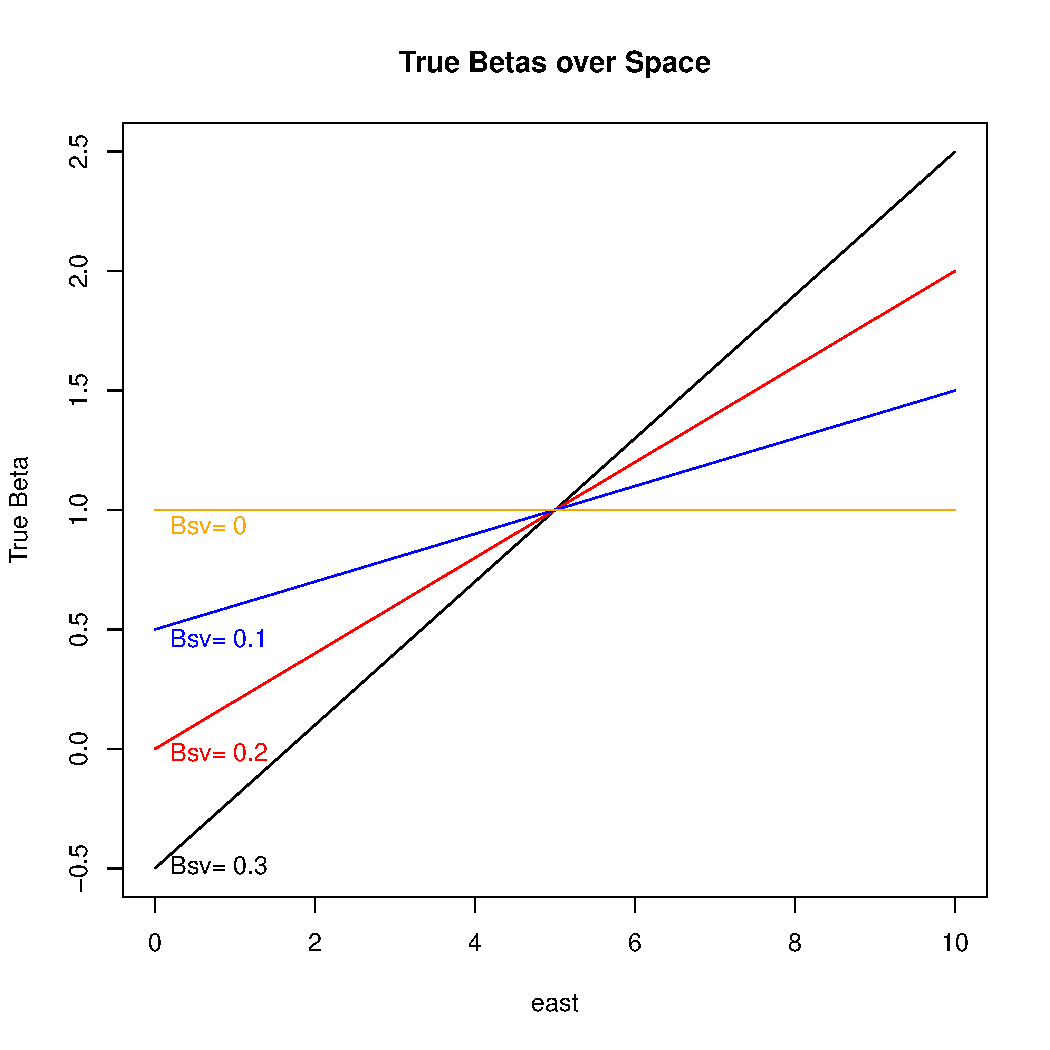
\includegraphics{figure/unnamed-chunk-4} 
\end{knitrout}


\section{Research Questions}

What do we want to know about LWR?

\begin{enumerate}
  \item Are there systematic differences in the bandwidth size selected by different techniques? How do LOOCV, Standardaized CV, Generalize CV, and the AICc compare?
  \item What sort of spatial variation in the coefficients is necessary relative to the error to need LWR?
  \item If there is no spatial relationship, will LWR default back to global OLS?
\end{enumerate}

\end{document}
